\chapter{Functioneel ontwerp SOUP API}\label{ch:impl soup api}
De SOUP API is de centrale module voor het systeem dat verantwoordelijk is voor het periodiek scannen van de projecten, het parsen van de rapporten die uit de analyses komt en het beschikbaar maken van de data die in de datbase is opgeslagen. In dit hoofdstuk wordt functioneel ingegaan op de werking van deze module en de drie sub modulen die ieders een deel van deze taken op zich neemt.


\section{API}\label{sec:api}
Centraal in de SOUP-API staat de API welke verantwoordelijkheid heeft om de data die door de beide Engines ,beschreven in het hoofdstuk Architectuur, worden verwerkt in goed banen te leiden. Om die reden zijn er twee controllers aangewezen die ieders

Om de data die in het datamodel (zie figuur~\ref{fig:SOUP-SoupApiDm} in het vorige hoofdstuk) gedefineerd is te bedienen is er gekozen om een generieke repository aan te maken die voor iedere service de basis bewerkingen verschaft. De business logica wordt gefineerd in de verschillende services die op zijn beurt weer aangeroepen worden door de overkoepelende datascontroller die voor de portal een mogelijkheid geeft om data in te zien en eventueel te bewerken.
\begin{figure}[bth]
    \myfloatalign
    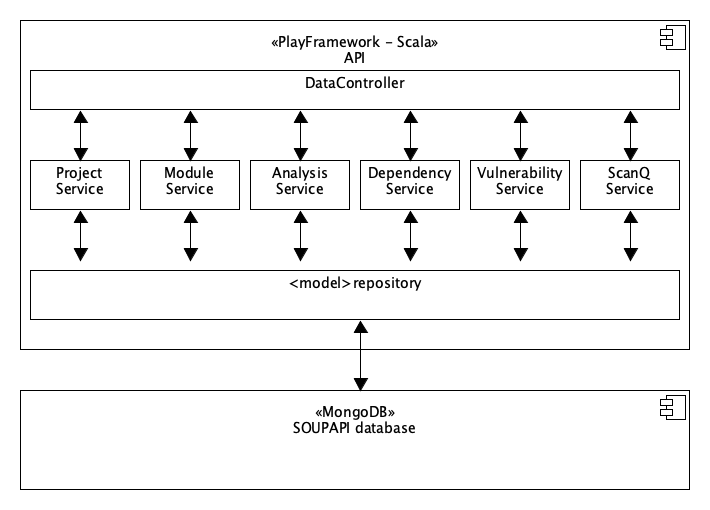
\includegraphics[width=12cm]{gfx/umlet/exports/API-ComponentsDiagram}
    \caption{API components }
    \label{fig:API components}
\end{figure}

Op deze manier is er een generieke manier waarop de database aan wordt gesproken. en er voor iedere model in het domein toch een individuele manier om met deze objecten op te gaan. DE controller is uitsluitend voor datatoegang voor buiten af, dit om ervoor te zorgen dat niet iedere data door elk component kan worden bewerkt.


\subsection{DataController}\label{subsec:datacontroller}
De datacontroller fungeert als een REST controller welke in staat steld om van buiten af toegang te krijgen tot informatie en waar gewenst aan te passen de volgende end-points worden gedefineerd waardoor de achterliggende services de business logica verzorgen en de gewenste data retourneren

\begin{itemize}
    \item Project Retourneert een Project Object RETOURWAARDEN AANGEVEN
        \begin{itemize}
            \item \textbf{GET: /data/project/} haalt alle projecten op zonder relaties
            \item \textbf{GET: /data/project/:id}
            \item \textbf{GET: /data/project/:name} get project by name
        \end{itemize}
    \item Module
    \begin{itemize}
        \item \textbf{GET: /data/module} get
        \item \textbf{GET: /data/module/:id} get project by ID
        \item \textbf{GET: /data/module/:name} get project by name
        \item \textbf{GET: /data/pro}
    \end{itemize}
    \item Analyses
    \begin{itemize}
        \item \textbf{GET: /data/analysis} get all projects
        \item \textbf{GET: /data/analysis/:id} get project by ID
        \item \textbf{GET: /data/analysis/:name} get project by name
    \end{itemize}
    \item dependency
    \begin{itemize}
        \item \textbf{GET: /data/dependency} get all projects
        \item \textbf{GET: /data/dependency/:id} get project by ID
        \item \textbf{GET: /data/dependency/:name} get project by name
    \end{itemize}
    \item Vulnerability
    \begin{itemize}
        \item \textbf{GET: /data/vulnerability} get all projects
        \item \textbf{GET: /data/vulnerability/:id} get project by ID
        \item \textbf{GET: /data/vulnerability/:name} get project by name
    \end{itemize}
\end{itemize}

AANVULLEN



De Api is verantwoordelijk voor de toegang tot de data is de database.
Er wordt een generic repo aangemaakt die het mogelijk maakt om voor verschillende objecten in het datamodel verschillende CRUD taken te doen. De business logica wordt in een eigen laag ondergebracht waarbij voor
%https://stackoverflow.com/questions/70513344/scala-generic-repository-class-for-reactive-mongo-repositoryalpakka-needed-c
De dataservice is verantwoordelijk voor het beschikbaar stellen en het onderhoud van de data in de database. Dit wodt bewerkstelligd door repositories aan te maken voor ieder model in het datamodel beschreven in het vorige hoofdstuk (zie figuur~\ref{fig:SOUP-SoupApiDm}) de repositories zijn verantwoordelijk voor de directe communicatie met de database.

\section{ReportParserEngine}\label{sec:reportparserengine}
De ReportParserEngine is verantwoordelijk voor het omzetten van een rapport dat gegenereerd wordt door een Software Composition Analysis Tool naar het interne datamodel. Het feit dat er veel tools zijn die allemaal de mogelijkheid hebben om projecten te analyseren op kwetsbaarheden en hier een rapport over uit kunnen brengen geeft al aan dat de ReportParserEngine is staat moet zijn om met verschillende rapporten van verschillende tools om moet kunnen gaan. Om dit te mogelijk te maken  is er gekozen voor een modulaire opzet waarbij er verschillende parsers geschreven kunnen worden die de rapporten kunnen omzetten. Deze Modulaire opzet is te zien in figuur~\ref{fig:ReportParserComponents} waarbij de $"$[FUTURE]Parser$"$ een placeholder is voor elke parser die in de toekomst moet worden tegevoegd om meerdere tools te ondersteunen.
\begin{figure}[bth]
    \myfloatalign
    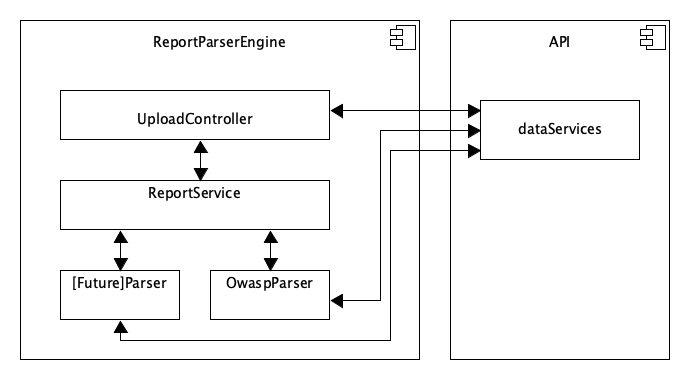
\includegraphics[width=12cm]{gfx/umlet/exports/ReportParserComponents}
    \caption{ReportParserEngine Components}
    \label{fig:ReportParserComponents}
\end{figure}
De


Het gehele process van het parsen van een rapport begint bij het uploaden van een rapport. Er zijn twee endpoints gediefineerd die ieder verantwoordelijk zijn voor een deel van het proces
In figuur~\ref{fig:SequenceClientUploadReport}

\subsection{UploadController}\label{subsec:uploadcontroller}
De controller fungeerd als gateway waar rapporten naar kunnen worden geupload. Het upload process is opgedeeld in twee delen waarbij er eerst een analyse wordt voorbereid, waarbij een nieuwe analyses wordt toegevoegd aan een module. Dit proces geeft een analyseToken terug dat gebruikt wordt om vervolgens het rapport aan de analyse toe te voegen.
\begin{figure}[bth]
    \myfloatalign
    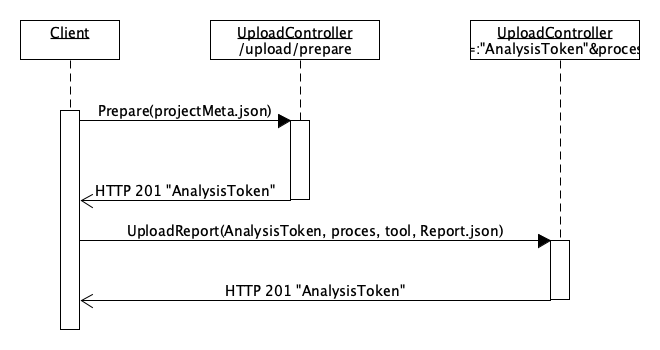
\includegraphics[width=12cm]{gfx/umlet/exports/SeqAddReport}
    \caption{Sequence upload to UploadController}
    \label{fig:SequenceClientUploadReport}
\end{figure}

\begin{itemize}
    \item \textbf{POST /upload/jenkins}: in de body worden de volgende bestanden verstuuurt: modulemeta.json , reports.json, dependencydeclaraites. ModuleMeta bevat informatie over de huidide staat van de module/

    De body bevat een jsonobject met daarin projectmeta data. Op het moment dat er een analyse aangemaakt is wordt er een analysetoken toegekend die gebruikt kan worden voor het verdere process.
    \item \textbf{POST /upload/pae} in de body zit het raport van de tool. Waarbij de parameter het proces aangeeft of Jenkins dan al niet Periodic Analysis Engine het rapport aanbied en de tool
\end{itemize}

\subsubsection{ModuleMeta.json}
een voorbeeld van de jsonbody voor prepare is te zien in ~\ref{lst:prepareJSONBody}
\begin{lstlisting}[caption={Datamodel vanuit Jenkins},label=lst:prepareJSONBody]
    {
        "projectName":"GroeiGids",
        "moduleName":"portal",
        "JenkinsScan": true,
        "JenkinsScan": true,
        "BuildHash": "fb5f5cb47bbd0cbf2f4771c55242fedbf41c5efc",
        "buildDate": "22-01-2022",
        "JenkinsBuildnr: "23",
        "NodeVersion": 14.5,
        "NPMVersion": 5.6.3
        "SBTVersion": , // alleen voor illustratie er wordt alleen versie informatie meegegeven over de platform van de module zelf.
        "ScalaVersion": ,
        "JavaVersion":,
  }
\end{lstlisting}

\subsection{ReportService}\label{subsec:reportservice}
Deze service ligt achter de uploadcontroller en heeft de volgende functies:
\begin{itemize}
    \item aanmaken van analyses zie figuur(~\ref{fig:analysisPrepare})
    \item selecteren van de juiste reportParser op basis van binnengekomen parameter"tool" zie figuur(~\ref{fig:selectReportParser})
    \item selecteren van het juiste path voor elk proces
\end{itemize}

Omdat er op dit moment in het ontwerp de mogelijkheid bestaat om middels twee processen een rapport aan te bieden zijn er in deze service twee functies die deze processen bedienen.
Het PeriodicAnalysisEngine proces bied een rapport aan welke geanalyseerd moet worden, daarintegen bied het jenkins process naast het rapport ook de dependencydeclaraties aan. Om een analyse te kunnen opslaan moet deze eerst worden aangemaakt volgende het sequence diagram in figuur~\ref{fig:ProcesPayload}
\begin{figure}[bth]
    \myfloatalign
    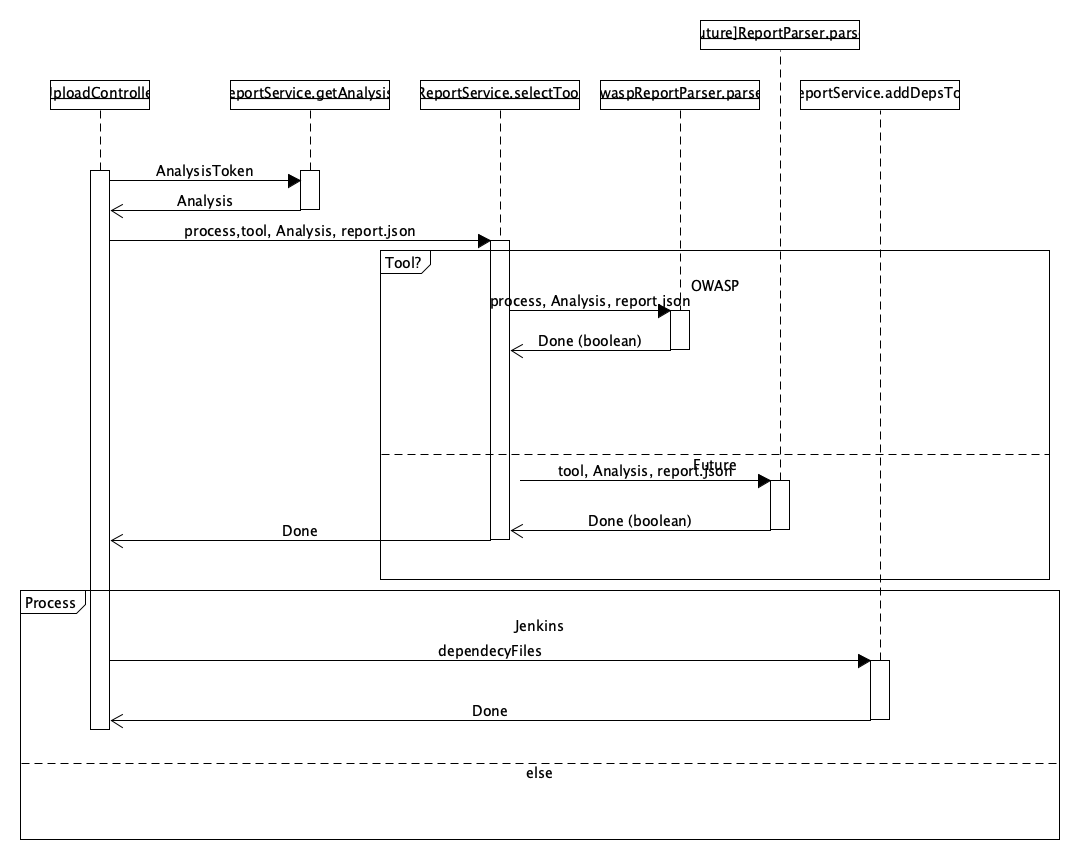
\includegraphics[width=14cm]{gfx/umlet/exports/SeqProcessPayload}
    \caption{Sequence diagram prepare Analysis}
    \label{fig:analysisPrepare}
\end{figure}

In het ontwerp is vastgelegt dat er altijd de mogleijkheid moet bestaan dat er tools toegevoegd kunnen worden aan de SOAP API. door dit mechanisme is dit mogelijk. Daarnasat moet er op het moment dat Jenkins de payload aanbied ook de dependencydeclaraties worden opgeslagen in de analyse.

\begin{figure}[bth]
    \myfloatalign
    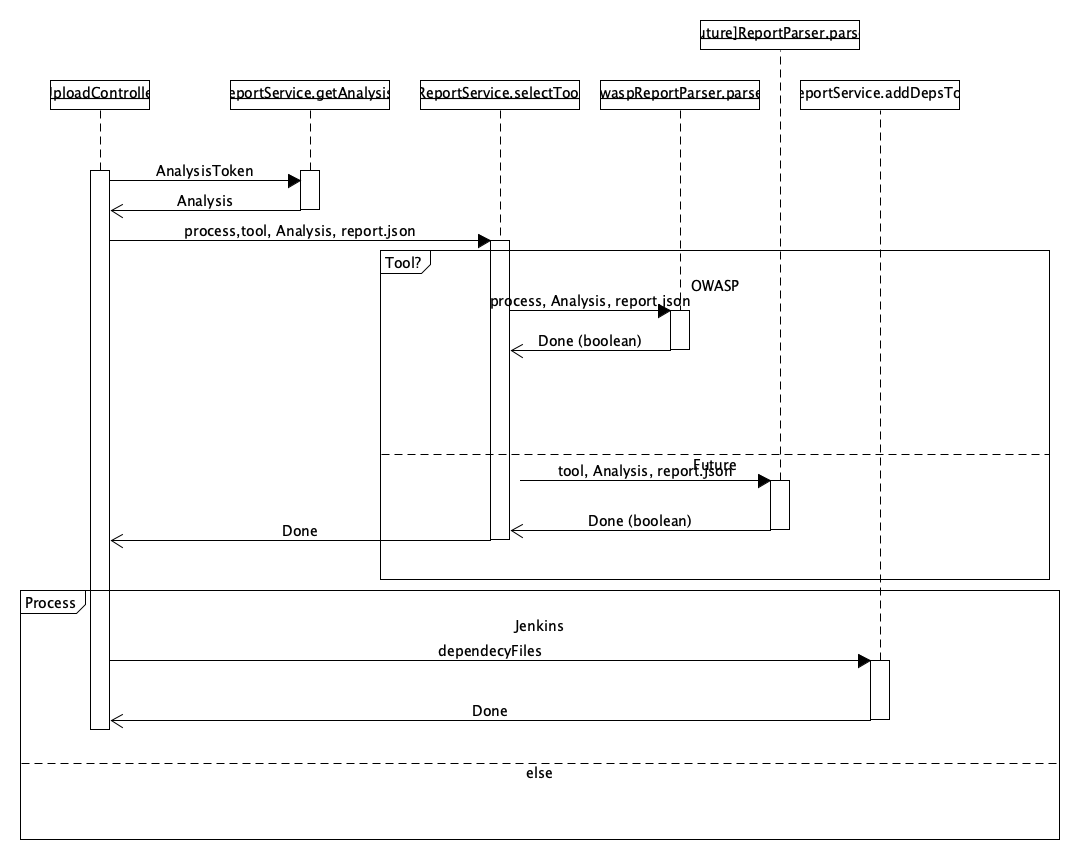
\includegraphics[width=14cm]{gfx/umlet/exports/SeqProcessPayload}
    \caption{Sequence diagram Proces Payload}
    \label{fig:ProcesPayload}
\end{figure}

\subsection{OWASP Parser}\label{subsec:owasp-parser}

\subsection{$"$[Future]Parser$"$}\label{subsec:$"$[future]parser$"$}
De $"$[Future]Parser$"$ zal in basis gelijk zijn als de parser voor de OWASP tool die hierboven worden beschreven. Echter zal de daadwerklijke omzetting veranderen. Om deze reden moet er voor iedere tool een eigen datamodel worden gedifineerd waarmee er objecten kunnen worden gemaakt van deze Data. Waarbij er vervolgens middels deze objecten naar het interne datamodel worden gewerkt.






\section{periodic anlalysisEngine}

\subsection{ScanQ}
De ScanQ is een lijst waarin alle analyses in geplanned staan. Bij deze lijst zijn een aantal functies de lijst beheren.

De datastructuur van de lijst is als volgt:
\begin{itemize}
    \item projectnaam: Naam van het project
    \item lastAnalyses: timestamp van de laatste analyse
    \item nestAnalyses: timestamp voor de volgende analyse
\end{itemize}





\section{SOUPAPI}\label{sec:soupapi}
De SOUP API is op zich zelf staande module binnen de SOUP-Analyses applicatie. Vanuit Eaglescience worden bijna alle applicaties middels Docker uitgerold en de SOUPAPI zal er geen uitzondering op zijn.

De SOUP API heeft drie hoofdtaken die ieder in een eigen service zijn gedefineerd. Welke middels DI aan elkaar zijn gelinkt.

maar samen werken om analyses beschikbaar te maken voor de portal:
\begin{itemize}
    \item ReportParser
    \item DataService
    \item Analyse controller
\end{itemize}





\section{AnalysisControlller}\label{sec:Implcontroller}
De controller is verantwoordelijk voor het aansturen van verschillende taken binnen de analyses van kwetsbaarheden binnen voor de soup module bekende projecten. Hieronder worden de verschillende onderdelen van deze controller en de relatie met elkaar verder uitgewerkt.

Eén van de belangrijkste taken van de controller is het bijhouden van de gevonden kwetsbaarheden binnen projecten en deze inzichtelijk maken voor de gebruiker. Er moet zowel inzicht komen op basis van project als op basis van Dependency

\section{ReportParser}



De Controller is verantwoordelijk voor de taken die te maken hebben met het periodiek scannen van projecten Het heeft faciliteiten zoals een scanQ waarin de projecten staan die gescanned moeten worden. Een analyser die op het moment dat een project aan de beurt is om geanalyseerd te worden een aantal subtaken sequentieel uitvert per module binnen een project.
In grote lijnen wordt er een dockercontainer opgezet per module waarin alle benodigde bestanden (dependency declaraties en dergelijke) worden geplaats. Vervolgens een analyse wordt uitgevoerf waaruit de resultaten naar de ReportParser kan worden gestuurt voor analyse. De exacte werking wpordt verderop in het document technisch uitgewerkt.




\subsection{Verwerking gegevens vanuit de builds}\label{subsec:verwerking-gegevens-vanuit-de-sca}
De belangrijkste taak van de SOUP API is het verwerken van de gegevens die beschikbaar worden gemaakt vanuit een analyse door de SCA Tooling en deze op te slaan in de database. De gegevens komen binnen van twee verschillende processen:
\begin{itemize}
    \item Jenkins buildstraat
    \item Intern periodiek scan systeem (nog betere naam vinden)
\end{itemize}

Het verschil tussen deze twee processen is dat er bij de data die binnenkomt bij Jenkins naast het rapport ook de dependency declataties zitten die later worden gebruikt om periodiek te kunnen analyseren. Het opbouwen van een analyse wordt gedaan in twee verscvhillende processen waarbij er bij aanvang van de analyse een prepare wordt uigevoerd wat ervoor zorgt dat een project, module en analyse zijn gevonden dan al niet aangemaakt om de analyse daadwerkelijk aan



In figuur(~\ref{fig:UploadReportFlow}) is te zien hoe een upload van een raport wordt verwerkt. Er is gekozen om twee endpoints aan te bieden voor de twee verschillende processen die verantwoordelijk zijn voor het aanleveren van een rapport. Eén endpoint waar het process binnen Jenkins het rapport.json en dependency declaraties kan verstuen en Eén endpoint waar het periodieke systeem het rapport kan versturen.
Beide endpoints bevatten Parameters om extra meta data mee te sturen die informatie bevatten over welkeproject/module het gaat. En in het geval van de jenkins endpoint ook de Githash waar jenkins de build voor heeft gedaan en het resulterende jenkinsBuildnummer. De laatst parameter die meegestuurd wordt is de selector voor de gebruikte tool waarmee de reportService de juiste parser kan kiezen.

Dit ontwerp is voorzien van een OWASPReportParser welke gebruikt kan worden om de rapporten gegenereerd door de OWASP tool om te zetten naar het interne datamodel. Door gebruik te maken van een tussenliggende service is het mogelijk om hier meerdere parsers aan toe te voegen zodat in de toekomst andere parsers geschreven kunnen worden die een rapport van een toekomstige tool om kan zetten in hetzelfde interne datamodel.
\begin{figure}[H]
    \myfloatalign
    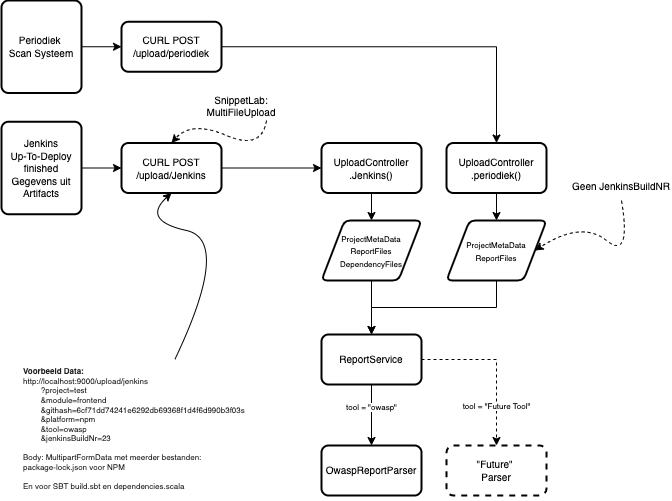
\includegraphics[width=10cm]{gfx/SOUPAPI-UploadAnalysis}
    \caption{Upload Report Flow}
    \label{fig:UploadReportFlow}
\end{figure}
Zoals eerder benoemd is de OWASP parser verantwoordelijk voor het inlezen van een aangeboden JSON en deze vervolgens op te slaan in een database op basis van het interne datamodel. Om dit te bewerkstelligen dienen de volgende stappen te worden genomen:
Als eerst wordt er gekeken of het in de parameters meegegeven project bestaat binnen de SOUPAPI. Als dit het geval is dan wordt er gekeken of de meegegeven module in het project bestaat. Mocht het project niet bestaan dan wordt er één aangemaakt samen met de meegegeven module en de default SOAPAPI projectsettings. Mocht de module niet bestaan dan wordt deze aangemaakt met de parameters die meegegeven zijn en vervolgens toegevoegd aan het project.
Op het moment dat zowel het project als de module bestaan wordt er een analyse aangemaakt en toegevoegd aan de
module. Als het een upload is vanuit het JenkinsProces worden de meegezonden dependency declaraties opgeslagen. Daarnaast wordt er voor iedere dependency in het rapport bekeken of deze al in de database staat. Als dit het geval is dan wordt deze toegevoegd aan de analyse. Als de dependency nog niet bestaat wordt deze opgeslagen in de database en vervolgens toegevoegd aan de analyse. Vervolgens wordt de vulnerability toegevoegd en gelinkt aan de dependencies. en ook hier geld als de vulnerability al bestaat is er alleen een link nodig.
Als laatst wordt er een nieuwe analyse toegevoegd aan de scanQ waarna er een result HTTP 200/201 komt.
\begin{figure}[H]
    \myfloatalign
    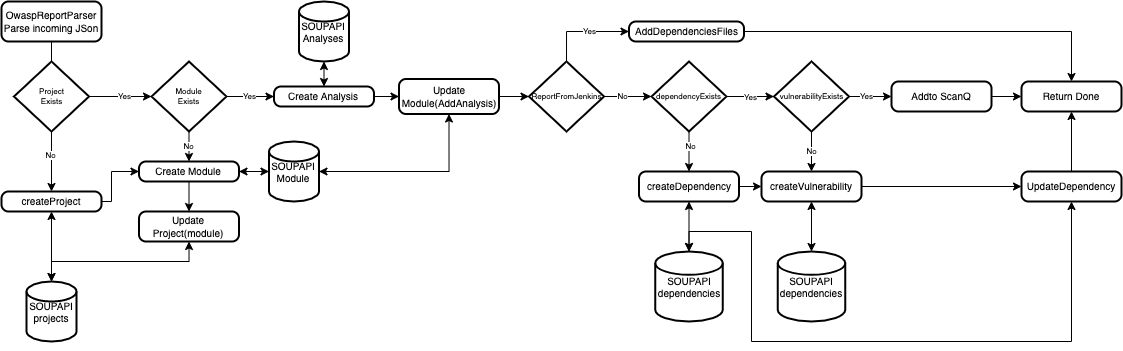
\includegraphics[width=15cm]{gfx/SOUPAPI-ReportParseFlow}
    \caption{Owasp Report Flow}
    \label{fig:OwaspReportFlow}
\end{figure}

\subsection{AnalysesController}\label{subsec:controller}
Naast de analyses die van de rapporten die uit het jenkins process komen is er ook behoefte om periodiek te analyseren op oudere niet actieve projecten. Om dit te kunnen faciliteren omnvat de Analyses controller een aantal componenten die ieders verantwoordelijk zijn voor een eigen taak:

\begin{figure}[H]
    \myfloatalign
    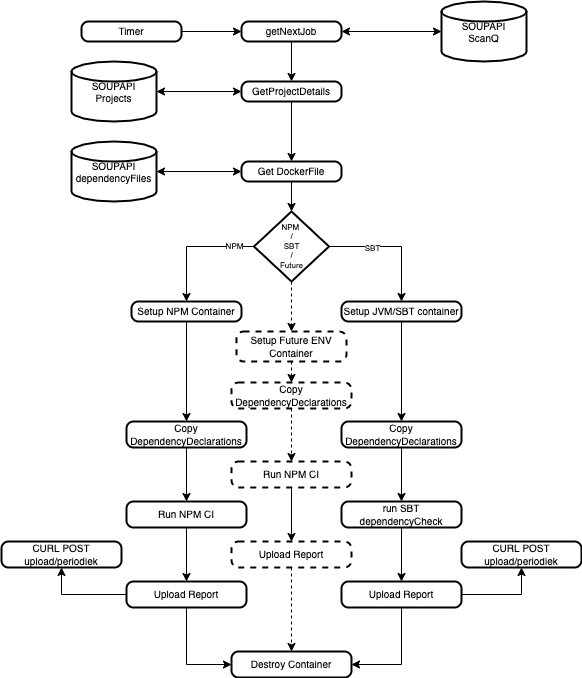
\includegraphics[width=10cm]{gfx/SOUPAPI-Periodic Analysis}
    \caption{Periodieke analyse flow}
    \label{fig:PeriodicAnalysis}
\end{figure}

\subsubsection{Timer}
De timer is verantwoordelijk voor het op tijd starten van de periodieke analyses op projecten die in de ScanQ staan. Op het moment dat er een geplannde analyse uitgevoerd moet worden zal deze aan de analyses controller worden gegeven die de verantwoordelijkheid overneemt.
\subsubsection{ScanQ + ScanQController}
De scanQ is een datastructuur gebasseerd op een list/seq waarin de analyses opgeslagen zijn die uitgevoerd moeten worden. De ScanQcontroller regelt de mutaties op deze scanQ.
\subsubsection{AnalysesController}
De analyse controller dient de taken uit te voeren die in figuur(~\ref{fig:PeriodicAnalysis}) weergegeven zijn. Dit is een sequenteel proces waarbij de controller wacht op antwoord voordat het een volgend onderdeel begint.



De rapporten uit het JenkinsProces vormen de basis van de analyse. Op het moment dat een analyse is toegevoegd worden ook de dependency declaraties opgeslagen. Deze declaraties vormen de basis voor de period

\subsection{API}\label{subsec:api}







